\documentclass{article}
%http://tex.stackexchange.com/a/196456/7712
\usepackage{tikz,etoolbox}
\usetikzlibrary{calc}

\makeatletter
\newcount\@eledtikzline
\@eledtikzline=1
\xdef\@eledtikzlines{}

\newcommand{\beledtikzline}{%
  \the\@eledtikzline%
}
\newcommand{\eeledtikzline}{%
  \xdef\@eledtikzlines{%
    \ifx\@eledtikzlines\empty%
      \the\@eledtikzline%
    \else%
      \@eledtikzlines,\the\@eledtikzline%
    \fi
    }%
  \global\advance\@eledtikzline by 1%
}
\def\lines{1,2,3}

\begin{document}

  \noindent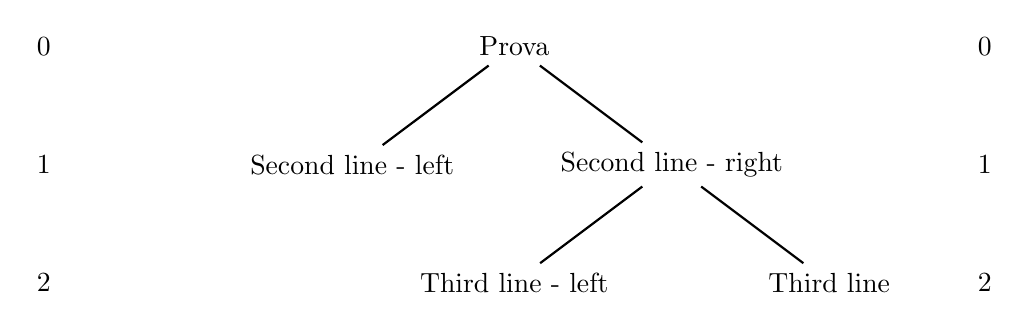
\begin{tikzpicture}[sibling distance=4cm,
                      edge from parent/.style={draw,thick}]

   \node(\beledtikzline){Prova\eeledtikzline}
        child {node[align=left] {Second line - left } }
        child {node(\beledtikzline)[align=right] {Second line - right\eeledtikzline}
            child {node (\beledtikzline)[align=left] { Third line - left}}
            child {node {Third line \eeledtikzline}}
        };

  
  \foreach \Node in \@eledtikzlines {%\y1=y-coord of the node
    \path let \p1=($ (\Node) $) in node at (0,\y1)[text width=\textwidth]{\Node\hfill\Node};
  }
\end{tikzpicture}


\noindent a\hfill main text\hfill b

\noindent a\hfill main text\hfill b

\end{document}